% 保留原始面板、实拍、示例与全部连线；仅以 TikZ 覆盖说明标签。
\begin{tikzpicture}
\node[anchor=south west,inner sep=0] (im) at (0,0) {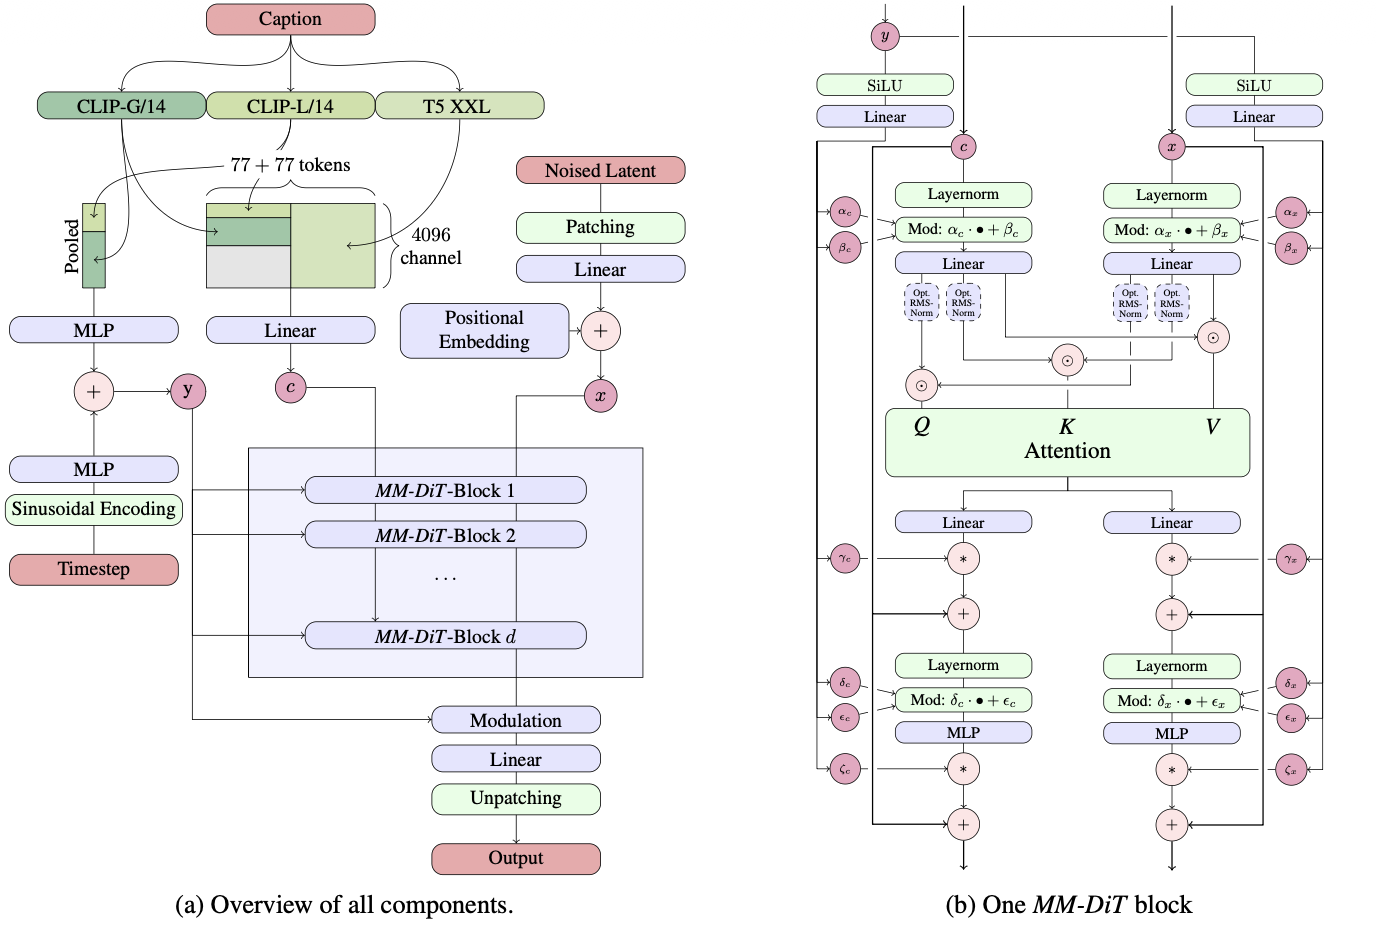
\includegraphics[width=\linewidth]{figures/stable.png}};
\begin{scope}[x={(im.south east)},y={(im.north west)}]
\fill[red!15] (0.153343,0.968017) rectangle (0.270349,0.992537);
\node[align=center,inner sep=0pt,font=\fontsize{8}{9}\selectfont,text width=0.117006\linewidth,rotate=0] at (0.211846,0.980277) {图像描述};
\fill[white] (0.159884,0.811301) rectangle (0.260901,0.837953);
\node[align=center,inner sep=0pt,font=\fontsize{7.5}{8.5}\selectfont,text width=0.101017\linewidth,rotate=0] at (0.210392,0.824627) {77 + 77 词元};
\fill[white] (0.287064,0.708955) rectangle (0.339390,0.764392);
\node[align=center,inner sep=0pt,font=\fontsize{7.5}{8.5}\selectfont,text width=0.052326\linewidth,rotate=0] at (0.313227,0.736674) {4096\\通道};
\fill[red!15] (0.378634,0.807036) rectangle (0.494913,0.831557);
\node[align=center,inner sep=0pt,font=\fontsize{8}{9}\selectfont,text width=0.116279\linewidth,rotate=0] at (0.436773,0.819296) {加噪潜变量};
\fill[green!8] (0.378634,0.745203) rectangle (0.494186,0.769723);
\node[align=center,inner sep=0pt,font=\fontsize{8}{9}\selectfont,text width=0.115552\linewidth,rotate=0] at (0.436410,0.757463) {分块};
\fill[blue!8] (0.378634,0.701493) rectangle (0.494186,0.726013);
\node[align=center,inner sep=0pt,font=\fontsize{8}{9}\selectfont,text width=0.115552\linewidth,rotate=0] at (0.436410,0.713753) {线性层};
\fill[blue!8] (0.295785,0.624733) rectangle (0.408430,0.672708);
\node[align=center,inner sep=0pt,font=\fontsize{8}{9}\selectfont,text width=0.112645\linewidth,rotate=0] at (0.352108,0.648721) {位置嵌入};
\fill[green!8] (0.007267,0.442431) rectangle (0.129360,0.470149);
\node[align=center,inner sep=0pt,font=\fontsize{7.5}{8.5}\selectfont,text width=0.122093\linewidth,rotate=0] at (0.068314,0.456290) {正弦编码};
\fill[red!15] (0.010174,0.380597) rectangle (0.125000,0.406183);
\node[align=center,inner sep=0pt,font=\fontsize{8}{9}\selectfont,text width=0.114826\linewidth,rotate=0] at (0.067587,0.393390) {时间步};
\fill[blue!8] (0.226017,0.465885) rectangle (0.421512,0.488273);
\node[align=center,inner sep=0pt,font=\fontsize{8}{9}\selectfont,text width=0.195494\linewidth,rotate=0] at (0.323765,0.477079) {MM-DiT 块 1};
\fill[blue!8] (0.226017,0.416844) rectangle (0.421512,0.439232);
\node[align=center,inner sep=0pt,font=\fontsize{8}{9}\selectfont,text width=0.195494\linewidth,rotate=0] at (0.323765,0.428038) {MM-DiT 块 2};
\fill[blue!8] (0.226017,0.308102) rectangle (0.421512,0.330490);
\node[align=center,inner sep=0pt,font=\fontsize{8}{9}\selectfont,text width=0.195494\linewidth,rotate=0] at (0.323765,0.319296) {MM-DiT 块 d};
\fill[blue!8] (0.317587,0.221748) rectangle (0.431686,0.243070);
\node[align=center,inner sep=0pt,font=\fontsize{8}{9}\selectfont,text width=0.114099\linewidth,rotate=0] at (0.374637,0.232409) {调制};
\fill[blue!8] (0.317587,0.178038) rectangle (0.431686,0.199360);
\node[align=center,inner sep=0pt,font=\fontsize{8}{9}\selectfont,text width=0.114099\linewidth,rotate=0] at (0.374637,0.188699) {线性层};
\fill[green!8] (0.317587,0.135394) rectangle (0.431686,0.156716);
\node[align=center,inner sep=0pt,font=\fontsize{8}{9}\selectfont,text width=0.114099\linewidth,rotate=0] at (0.374637,0.146055) {还原分块};
\fill[red!15] (0.317587,0.072495) rectangle (0.431686,0.093817);
\node[align=center,inner sep=0pt,font=\fontsize{8}{9}\selectfont,text width=0.114099\linewidth,rotate=0] at (0.374637,0.083156) {输出};
\fill[white] (0.039971,0.696162) rectangle (0.060320,0.771855);
\node[align=center,inner sep=0pt,font=\fontsize{6.5}{7.5}\selectfont,text width=0.020349\linewidth,rotate=0] at (0.050145,0.734009) {池\\化};
\fill[blue!8] (0.596657,0.868870) rectangle (0.691134,0.884861);
\node[align=center,inner sep=0pt,font=\fontsize{7.5}{8.5}\selectfont,text width=0.094477\linewidth,rotate=0] at (0.643895,0.876866) {线性层};
\fill[blue!8] (0.864826,0.868870) rectangle (0.956395,0.884861);
\node[align=center,inner sep=0pt,font=\fontsize{7.5}{8.5}\selectfont,text width=0.091570\linewidth,rotate=0] at (0.910610,0.876866) {线性层};
\fill[blue!8] (0.654797,0.711087) rectangle (0.747820,0.728145);
\node[align=center,inner sep=0pt,font=\fontsize{7.5}{8.5}\selectfont,text width=0.093023\linewidth,rotate=0] at (0.701308,0.719616) {线性层};
\fill[blue!8] (0.805959,0.711087) rectangle (0.899709,0.728145);
\node[align=center,inner sep=0pt,font=\fontsize{7.5}{8.5}\selectfont,text width=0.093750\linewidth,rotate=0] at (0.852834,0.719616) {线性层};
\fill[blue!8] (0.654797,0.433902) rectangle (0.747820,0.450959);
\node[align=center,inner sep=0pt,font=\fontsize{7.5}{8.5}\selectfont,text width=0.093023\linewidth,rotate=0] at (0.701308,0.442431) {线性层};
\fill[blue!8] (0.805959,0.433902) rectangle (0.899709,0.450959);
\node[align=center,inner sep=0pt,font=\fontsize{7.5}{8.5}\selectfont,text width=0.093750\linewidth,rotate=0] at (0.852834,0.442431) {线性层};
\fill[green!8] (0.651163,0.777186) rectangle (0.750727,0.805970);
\node[align=center,inner sep=0pt,font=\fontsize{7.5}{8.5}\selectfont,text width=0.099564\linewidth,rotate=0] at (0.700945,0.791578) {层归一化};
\fill[green!8] (0.803052,0.777186) rectangle (0.902616,0.805970);
\node[align=center,inner sep=0pt,font=\fontsize{7.5}{8.5}\selectfont,text width=0.099564\linewidth,rotate=0] at (0.852834,0.791578) {层归一化};
\fill[green!8] (0.651163,0.276119) rectangle (0.750727,0.304904);
\node[align=center,inner sep=0pt,font=\fontsize{7.5}{8.5}\selectfont,text width=0.099564\linewidth,rotate=0] at (0.700945,0.290512) {层归一化};
\fill[green!8] (0.803052,0.276119) rectangle (0.902616,0.304904);
\node[align=center,inner sep=0pt,font=\fontsize{7.5}{8.5}\selectfont,text width=0.099564\linewidth,rotate=0] at (0.852834,0.290512) {层归一化};
\fill[green!8] (0.652616,0.742004) rectangle (0.686047,0.769723);
\node[align=center,inner sep=0pt,font=\fontsize{6}{7}\selectfont,text width=0.033430\linewidth,rotate=0] at (0.669331,0.755864) {调制};
\fill[green!8] (0.803779,0.742004) rectangle (0.837209,0.769723);
\node[align=center,inner sep=0pt,font=\fontsize{6}{7}\selectfont,text width=0.033430\linewidth,rotate=0] at (0.820494,0.755864) {调制};
\fill[green!8] (0.652616,0.240938) rectangle (0.686047,0.268657);
\node[align=center,inner sep=0pt,font=\fontsize{6}{7}\selectfont,text width=0.033430\linewidth,rotate=0] at (0.669331,0.254797) {调制};
\fill[green!8] (0.803779,0.240938) rectangle (0.837209,0.268657);
\node[align=center,inner sep=0pt,font=\fontsize{6}{7}\selectfont,text width=0.033430\linewidth,rotate=0] at (0.820494,0.254797) {调制};
\fill[blue!5] (0.656977,0.656716) rectangle (0.682413,0.699360);
\node[align=center,inner sep=0pt,font=\fontsize{5}{6}\selectfont,text width=0.025436\linewidth,rotate=0] at (0.669695,0.678038) {RMS};
\fill[blue!5] (0.689680,0.656716) rectangle (0.715116,0.699360);
\node[align=center,inner sep=0pt,font=\fontsize{5}{6}\selectfont,text width=0.025436\linewidth,rotate=0] at (0.702398,0.678038) {RMS};
\fill[blue!5] (0.808140,0.656716) rectangle (0.833576,0.699360);
\node[align=center,inner sep=0pt,font=\fontsize{5}{6}\selectfont,text width=0.025436\linewidth,rotate=0] at (0.820858,0.678038) {RMS};
\fill[blue!5] (0.840116,0.656716) rectangle (0.865552,0.699360);
\node[align=center,inner sep=0pt,font=\fontsize{5}{6}\selectfont,text width=0.025436\linewidth,rotate=0] at (0.852834,0.678038) {RMS};
\fill[green!8] (0.739099,0.503198) rectangle (0.820494,0.529851);
\node[align=center,inner sep=0pt,font=\fontsize{8}{9}\selectfont,text width=0.081395\linewidth,rotate=0] at (0.779797,0.516525) {注意力};
\fill[white] (0.123547,0.007463) rectangle (0.474564,0.050107);
\node[align=center,inner sep=0pt,font=\fontsize{8.5}{9.5}\selectfont,text width=0.351017\linewidth,rotate=0] at (0.299055,0.028785) {（a）全部组件概览};
\fill[white] (0.650436,0.001066) rectangle (0.987645,0.050107);
\node[align=center,inner sep=0pt,font=\fontsize{7.5}{8.5}\selectfont,text width=0.337209\linewidth,rotate=0] at (0.819041,0.025586) {（b）一个 MM-DiT 块\\虚线小框：可选 RMS 归一化};
\fill[blue!8] (0.153343,0.636461) rectangle (0.268895,0.660981);
\node[align=center,inner sep=0pt,font=\fontsize{8}{9}\selectfont,text width=0.115552\linewidth] at (0.211119,0.648721) {线性层};
\end{scope}
\end{tikzpicture}
